\chapter{Tecnología en el Proceso Electoral}
\label{SistemaElectoral}
\cambiar{No se describen todos los sistemas de votos existentes, y si se hace, están en forma muy resumida. No analiza ventajas y desventajas de cada uno (2.1.1). No se analizan los votos en papel sin uso de tecnología.}
\cambiar{Se habla de Boleta única de sufragio (BUS), Boleta única, Boleta única electrónica (BUE), boleta única en papel, etc. pero no se describe ninguna.}
\cambiar{Describe mecanismos de voto electrónico, pero no con sus características, sino con ejemplos de implementación. Deberían ser dos cosas diferentes.}
\cambiar{Faltan referencias que respalden los conceptos plasmados y las opiniones. En general se dan muchas opiniones, en su mayoría negativas, de los sistemas electorales nombrados sin fundamentos. Es decir, son opiniones del autor? se han analizado?}
\cambiar{A veces dice Figura, otras Gráfico, otras Imágen. Unificar Figura.}
\cambiar{En general: El capítulo advierte de una revisión conceptual de las características de un sistema electoral tradicional (según Capítulo 1). Sin embargo, luego se mezcla con la aplicación de tecnologías al sistema. No analiza y compara los sistemas de votos. Da opiniones sin fundamento.}

Involucrar tecnología en el proceso electoral es complejo, no sólo por sus desafíos técnicos, sino también por su importancia para el Estado y para la sociedad en general. Un sistema de voto electrónico involucra considerar aspectos de software, hardware, procesos operativos, y personas. Por lo tanto, cualquier desarrollo debe tener el aspecto de calidad como el objetivo más importante en el proceso.\newline
%\agregar{cita a texto del Ministerio - ESTO SALIÓ DEL DOCUMENTO DE CONICET Un sistema de votación debe considerar los siguientes objetivos \cite{conicet}: - HECHO}
Un sistema de votación debe considerar los siguientes objetivos \cite{conicet}:
\begin{itemize}
    \item Garantizar la completitud en la oferta electoral
    \item Simplificar el uso de boletas (por ej. con boleta única)
    \item Brindar mayor accesibilidad a los ciudadanos a la hora de votar (por ej. para personas con alguna discapacidad)
    \item Lograr precisión y rapidez en el proceso de conteo de votos
\end{itemize}
Además un sistema de votación que incorpore algún grado de automatización debe construir la confianza de los ciudadanos, partidos políticos y gobierno, en el sistema y en el proceso de votación \cite{conicet}.

Una de las ventajas más deseadas en automatizar el proceso es la rapidez en el conteo. Si todo sale bien los resultados pueden ser inmediatos pero el problema es el impacto que pueden generar las distintas ``cosas'' que pueden salir mal. La rapidez sin confianza ni seguridad no es útil para cualquier proceso electoral y por esto es que la eficacia debe importar por sobre la eficiencia o rapidez.

\section{Sistema electoral}

Un sistema electoral consiste de reglas y procedimientos técnicos que producen determinadas consecuencias, es decir, los sistemas electorales no son neutros. 
La complejidad es afectada por la cantidad de representantes que se eligen por distrito electoral y la forma de votación. El voto se realiza a través de las boletas electorales, las cuales son el instrumento por el cual el ciudadano expresa su voluntad, además de ser la prueba real del voto y el medio para realizar el recuento de votos o escrutinio.
Actualmente las condiciones jurídicas del sufragio están constituidas por su universalidad, igualdad, obligatoriedad y secreto. Sin embargo, en Argentina para llegar a ese punto, los condicionamientos y las formas de votar fueron modificándose a través de la historia \cite{historia}.\newline

Desde 1873 que el voto oral se convirtió en un voto escrito, fue modificándose hasta conseguir que en 1995, por la reforma de la Constitución Nacional queda hasta el día de la fecha el régimen electoral como el siguiente:
\begin{itemize}
    \item Sistema de Representación Proporcional
    \item Método de Conversión de votos en escaños: Sistema D'Hondt
    \item Umbral 3\% del padrón electoral de distrito
    \item La elección de todos los representantes argentinos se eligen en forma directa por el pueblo de la Nación Argentina.
\end{itemize}
\newline





\subsection{Clasificación de Sistemas de Voto Electrónico}
%\cambiar{En el sistema electoral existen partes del proceso vulnerables a la incorporación de recursos informáticos con el objetivo de agilizar su ejecución. Como concepto general, se considera voto electrónico a todo sistema electoral que agregue tecnología a las fases de emisión y recuento de votos de la mesa de votación. Hay experiencias de implementación de voto electrónico distintos puntos del país y en otros países, utilizando variadas técnicas y con diferentes niveles de aceptación.  En algunos casos se logró la implantación de el voto electrónico y en otros luego de unos cuantos intentos se volvió al sistema electoral tradicional.\newline Se identifican 3 grandes mecanismos:  - HECHO}


En el sistema electoral existen partes del proceso vulnerables a la incorporación de recursos informáticos con el objetivo de agilizar su ejecución. Como concepto general, se considera voto electrónico a todo sistema electoral que incorpore tecnología en las fases de emisión y durante el recuento de votos de la mesa de votación. Experiencias de implementación de voto electrónico en distintos puntos del país y en otros países utilizaron variadas técnicas con distintos impactos de aceptación o rechazo logrando unos cuantos intentos para finalmente volver al sistema electoral tradicional.\newline
Se identifican 3 grandes mecanismos:
\begin{itemize}
    \item Los sistemas de recuento automático de votos mediante reconocimiento óptico de marcas aplicadas en la boleta por parte de los ciudadanos.	Los primeros sistemas datan del siglo XIX en Nueva York mediante tarjetas perforadas. En Venezuela (1994 – 2003) implementaron el sistema mediante boletas impresas en papel que luego el elector debía rellenar para luego ser contabilizado mediante reconocimiento óptico de caracteres \cite{eleccionesVenezuela}.\newline
    \underline{Ventajas:} Mantener el principio de que la voluntad del elector se mantiene en un trozo de papel anónimo fácilmente auditable independiente de los dispositivos y software usados.\newline
    \underline{Desventajas:} Suponen un doble trabajo para el votante (elegir y además controlar que su elección sea correctamente impresa). Pone en riesgo el anonimato del voto al poder agregar “suciedad” que en realidad codifique información que permita reconstruir la emisión de los votos y la relación de cada votante con su voto.\newline
    \underline{Conclusión:} Si bien cualquier sistema basado en papel podría ser adulterado, esto debe ser hecho individualmente con cada boleta, y el impacto de una persona corrupta se limita a las boletas bajo su custodia. En el sistema electrónico, en cambio, una única persona corrupta tiene el potencial de influenciar sobre un gran número de máquinas, comprometiendo la integridad de votos en masa, incluyendo los de las mesas cuyos fiscales actúen de buena fe.
    \item Los sistemas de registro electrónico directo (DRE) – urnas electrónicas. En Brasil, varios estados de EEUU y las últimas elecciones de Venezuela implementaron el sistema DRE. Esta realiza simultáneamente el registro y la tabulación del voto mediante un dispositivo informático, operado directamente por el votante (teclado, botonera o teclado táctil), registrándose el voto directamente en la memoria del dispositivo.\newline
    \underline{Ventajas:} Elimina por completo el uso de papel, no hay boletas que custodiar.\newline
    %\cambiar{cv lo siguiente no esta claro que sea una desventaja. Habria que poner por ejemplo. No permite la anulacion del voto como expresión democratica del votante o algo asi }
    \underline{Desventajas:} No permite la anulación del voto como medio de expresión democrática del votante. Además dificulta la fiscalización de la integridad del voto al no existir una separación entre el votante y el escrutinio, por lo tanto, poder reconocer una falla o un error es muy difícil de descubrir a tiempo. \newline
    \underline{Conclusión:} Genera un punto de tensión entre los ciudadanos que necesitan que el resultado refleje sus elecciones y los encargados de conducirlos que desean terminar la tarea con mayor rapidez y menor esfuerzo delegando la mayor responsabilidad que se pueda por posibles errores o actos de corrupción.
    %\agregar{cv: creo que aquí hay que enfatizar la dificultad de la fiscalización de la integridad del voto, es el caso extremo en ese sentido - HECHO}
    %\agregar{pk: cita a sistema de votación utilizado en Debian \url{https://www.debian.org/vote/} - HECHO}
    %\cambiar{pk: Los sistemas de votación a distancia a través de Internet, como el sistema devotee utilizado utilizado para elegir para votar en el Proyecto Debian... - HECHO}
    \item Los sistemas de votación a distancia a través de Internet, como el sistema DEbian VOTe EnginE (devotee) utilizado como un sistema de votos en el Proyecto Debian \footnote{Proyecto Debian: \url{https://www.debian.org/vote/}} es un proyecto comunitario con excelentes resultados de uso. El sistema es robusto, justo y difícil de engañar, pero solo funciona gracias al hecho de que el voto no es secreto.\newline
    \underline{Desventajas:} Identificar que un votante solo vote una única vez o impedir que vote a nombre de otra persona, o no esté habilitado para votar, a diferencia de la verificación presencial de los documentos de identidad por parte de autoridades electorales. Por lo tanto, estos sistemas obligan a que la máquina que recibe el voto tenga conocimiento de quien lo está emitiendo, generando un punto de ataque para quien quiera violar el secreto del voto.
\end{itemize}


\section{Propiedades de Calidad}
\cambiar{Sección 2.2. No están claras las propiedades nombradas. No las explica, sino que las compara con sistemas que no fueron descriptos.}
Para lograr un sistema electoral exitoso y confiable a la vista de las partes involucradas es necesario que cumpla ciertas propiedades de calidad, sin tener en cuenta si este proceso incluye tecnología o no. A continuación se enumeran estas propiedades que todo sistema electoral debe satisfacer.
%\agregar{Párrafo marco sobre Atributos de Calidad - HECHO?}
%\cambiar{A partir de las partes involucradas en el proceso surgen distintas propiedades a satisfacer un sistema electoral con o sin tecnología, que se describen a continuación. - HECHO}


\subsection{Secreto del voto}
Únicamente el votante debe poder tener conocimiento alguno del contenido del voto. La sola sospecha de que alguien pueda conocer el contenido de su voto impide la libre emisión del sufragio.
%\cambiar{Una experiencia de implementación de urna electrónicas en el estado de Ohio, EEUU ** año y cita ***** que vulneró el secreto del voto,  dos años después de haberlas usado, se descubrió que el sistema permitía reconstruir el vinculo entre el voto y el votante, a través de un reporte emitido por la urna al final del recuento - NO TENGO FECHA 2007 \url{https://en.wikipedia.org/wiki/Electronic_voting_in_the_United_States#Ohio}  \url{https://nordicinnovationlabs.com/wp-content/uploads/2018/07/everest.pdf} - HECHO}
Una experiencia de implementación de urna electrónica en el estado de Ohio, EEUU en el año 2007 que permitió eliminar el voto en cadena pero, se descubrió dos años después de haberlas usado, una falla grave en estas urnas que permitía reconstruir el vínculo entre el voto y el votante, a través de un reporte emitido por la urna al final del recuento \cite{mcdaniel2007everest}.

\subsection{Integridad}
%\agregar{Al caso de Holanda citar años - HECHO}
Requiere garantizar que la cadena de confianza no puede romperse. Esta propiedad también se encuentra ligada a la seguridad del sistema para proteger datos e información de accesos no autorizados, pero proveyendo al mismo tiempo acceso a personal autorizado para operar. En particular, se consideran importantes las propiedades de confidencialidad, integridad, disponibilidad y autenticidad. Los aspectos de Seguridad Informática cobran gran importancia en un sistema de misión crítica, un error en el sistema que pueda ser explotado por un atacante podría atentar contra alguno de los principios básicos del voto o el resultado de la votación en general. Frente a esto, tenemos el ejemplo de las elecciones en Holanda que a partir de 1997 se votaba con el sistema fabricado por la empresa Nedap. Luego de 9 años un grupo de activistas demostró en un programa de televisión las vulnerabilidades del sistema. Esto generó que el gobierno decidiera volver al sistema tradicional en papel \cite{eleccionesHolanda}. 
%\cambiar{pk:Otro ejemplo es el de las elecciones presidenciales?????? de EEUU en 2004,.. - HECHO}
Otro ejemplo serian las elecciones presidenciales de EEUU, como en el 2004 y las últimas elecciones en el 2020, en las que las diferencias entre las encuestas en boca de urna y los resultados finales sugieren fuertemente que las urnas dieron resultados dudosos.\newline
Esta propiedad incluye capturar la intención del voto de manera fehaciente (y sin introducir sesgos), registrar la intención de voto exactamente como fue capturada, garantizando que se respeta la voluntad de cada votante, es decir que el sistema no permita cambiar el voto una vez que el votante lo emitió, y contabilizar el voto exactamente como fue registrado. Si el sistema, por error o ataque, altera la suma de los votos individuales lo hará de una forma que será evidente para los ciudadanos.

\subsection{Capacidad de auditoría y control del proceso electoral (sin afectar los atributos de secreto e integridad anteriores)}
Capacidad de monitorear el sistema tanto en su diseño (estructura), como cuando se encuentra en funcionamiento (ejecución) y cuando ya dejó de utilizarse (análisis post-hoc). Un sistema de votación debe poderse auditar en todos los niveles de hardware y software. El principio rector es que 
%\agregar{pk: Agregar cita textual, si las comillas implican esto - CONICET O  (Benaloh, Ryan, Schneider & Teague, 2017)??}
``las elecciones deben dar una evidencia consistente de un resultado preciso, aún cuando el rival sea quien escribe el software, administra la elección o gobierna el país''.\newline
En el sistema de votación tradicional, la responsabilidad de auditoría está distribuida en todos porque todos pueden ver y entender el sistema. Lejos de aportar transparencia, la urna electrónica obstaculiza la capacidad de la mayoría de los ciudadanos de fiscalizar la elección, ya que queda necesariamente en manos de una élite tecnológica a la que el resto de la población no le queda otra que creerle.
%\cambiar{Este fue el caso de las de Georgia EEUU **citar año**, en las que las elecciones fueron cien por ciento electrónicas y con el mismo tipo de máquinas. Esto quiere decir que gran parte de los votos no tiene recuento posible ya que no existe comprobante físico para contabilizar \cite{eleccionesGeorgia}.\newline - HECHO}

Este fue el caso del estado de Georgia en EEUU que a partir del 2002 y hasta el 2019 las elecciones fueron cien por ciento electrónicas y con el mismo tipo de máquinas. Esto quiere decir que gran parte de los votos no tiene recuento posible ya que no existe comprobante físico para contabilizar \cite{eleccionesGeorgia}.\newline
La incorporación de urnas electrónicas tiene efectos contrarios a este objetivo ya que las personas con poca afinidad con los sistemas computacionales (adultos mayores, personas de escasos recursos, con dificultad visual, entre otras) se verán enfrentados a un sistema mucho más complejo para votar. Por otra parte, las personas que auditan las elecciones (maestras de escuela, empleados públicos, fiscales de partidos políticos) se verán incapaces de auditar eficazmente este tipo de sistema. Sólo un grupo reducido de personas relacionadas al área de sistemas computacionales comprenderán el funcionamiento de estos sistemas, pero dificilmente se atreverán a firmar a conciencia una certificación de seguridad de las urnas pues, no existe método formal de validación que los avale. Si bien no existen sistemas perfectos, la diferencia de impacto es sustancial. Un error mínimo en un sistema de votación electrónica puede alterar el resultado de una elección en un gran número de mesas simultáneamente.

%\cambiar{Agregué la imagen de las elecciones de neuquén - HECHO}
%\cambiar{Mover todas las imágenes a la carpeta img -HECHO}
\subsection{Igualdad de condiciones para todos los partidos políticos}
Todo sistema electrónico tiene un límite técnico donde manipular o visualizar la oferta electoral. Como ejemplo tenemos las elecciones del 2019 que se llevaron a cabo en Neuquén y Plottier para los comicios municipales (como muestra la Figura \ref{graf:buenqn}). En el caso de Plottier se debieron distribuir 29 listas en una pantalla con capacidad de 18 casilleros. Lograr distribuir la totalidad de las listas implicó que no exista ventaja entre candidatos por las maniobras de mercantilizar la herramienta de las colectoras \cite{limiteColectoras}.

\begin{figure}[h!]
    \begin{center}
        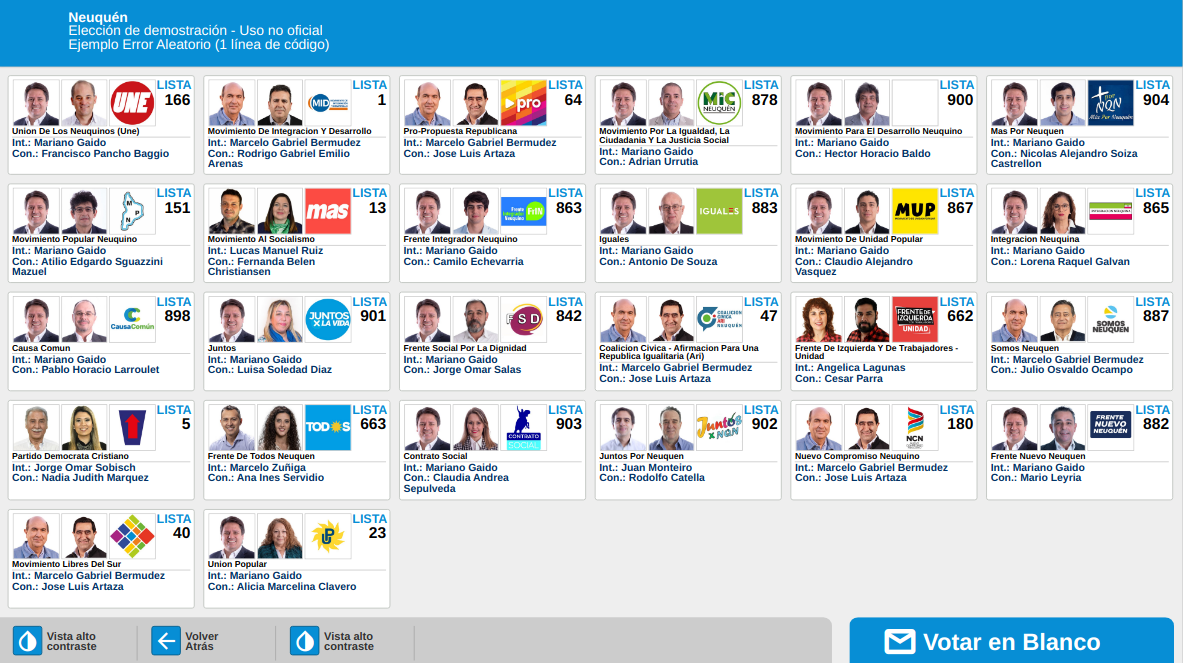
\includegraphics[width=\textwidth]{img/buenqn2019.png}
    \end{center}
  \caption{Pantalla del sistema BUE utilizado en las Elecciones Municipales de Neuquen 2019}
  \label{graf:buenqn}
\end{figure}

\subsection{Universalidad}
El sistema debe estar preparado para facilitar el sufragio de toda persona habilitada, esto incluye personas con requerimientos de accesibilidad, por ej. no videntes. Debemos tener en cuenta que toda persona posee los mismos derechos sobre el voto. Por lo tanto, si se requiere el acompañamiento debido a la complejidad o inaccesibilidad del sistema no se está alcanzando ninguna ventaja por sobre el sistema electoral tradicional.\newline
Como ejemplo, las máquinas usadas en elecciones electrónicas en general se basan en fotos y colores como medio de accesibilidad para las personas que no puedan leer o con baja visión. Por otro lado, en varios paises es común la instalación de un kit accesible como un teclado especial y auriculares para personas invidentes.

\subsection{Usabilidad}
%\cambiar{El sistema debe ser fácil y adecuado para toda persona involucrada en el proceso de la elección. Un sistema electrónico debe ser fácil de aprender tanto para un votante como para las autoridades encargadas de dar soporte. Esta propiedad también ayuda al objetivo de rapidez, ya que un sistema difícil de entender generará largas colas de espera para votar debido a que varias personas les lleva más tiempo entender y generar su sufragio. Así mismo la facilidad de uso mejoraría los tiempos del escrutinio realizado por las autoridades de mesa. - HECHO}

El sistema debe ser fácil e intuitivo para cualquier persona involucrada en el proceso de la elección. Un sistema electrónico debe ser fácil de aprender tanto para un votante como para las autoridades encargadas de dar soporte. Esta propiedad también ayuda al objetivo de rapidez ya que un sistema difícil de entender generará largas colas de espera para votar debido a que varias personas les lleva más tiempo entender y generar su sufragio. De igual manera la facilidad de uso mejoraría los tiempos del escrutinio realizado por cada autoridad de mesa.

\subsection{Cumplir con las normativas vigentes del proceso electoral}
Un sistema electoral regularmente no modifica sus políticas o reglas que lo conforman. De todos modos, un sistema de votación electrónica debe ser capaz de adaptarse a cualquier cambio adoptado por las autoridades de un país, provincia o distrito.

\subsection{Integridad vs. Auditabilidad vs. Secreto}
%\agregar{Agregar cita - HECHO}
En todo sistema electoral (sea en formato de papel o electrónico) se ha demostrado que satisfacer los atributos de integridad, auditabilidad y secreto simultáneamente es complejo y es una tarea imposible de cumplir. Cualquier sistema de voto electrónico que intente solucionar los problemas inherentes a garantizar integridad y secreto, estará en una situación difícil para lograr una verificación formal y en auditabilidad. \cite{conicet}

\section{Modelo de Referencia}
\cambiar{Sección 2.3: La Fig 2.2 presenta un circuito de 5 etapas para el proceso electoral. Debería nombrar en cada caso donde es aplicada la tecnología. Falta describir la etapa 5
(Procesamiento de resultados y publicación).}
\cambiar{Las subsecciones del modelo de referencia deben tener el mismo nombre. (Conteo →
Escrutinio de la Mesa)}
Mediante el análisis realizado por el Conicet \cite{conicet}, el sistema de votación se puede determinar en cinco fases secuenciales del proceso susceptibles de ser automatizada (Figura \ref{graf:modeloReferencia}) . Las fases están derivadas del Código Electoral Nacional (Decreto nº2135, 1983) \cite{decreto}
%\agregar{cita al Decreto}
%\agregar{artículo del CONICET - HECHO}

\begin{figure}[h!]
    \begin{center}
        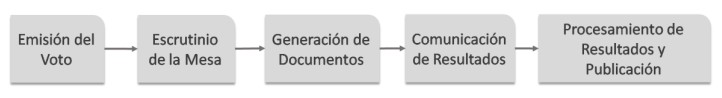
\includegraphics[width=\textwidth]{img/modeloReferencia.png}
    \end{center}
  \caption{Modelo de Referencia}
  \label{graf:modeloReferencia}
\end{figure}

%\agregar{Agregar imágen del modelo de referencia - HECHO}
%\cambiar{Está muy textual del artículo del CONICET (Modelo de Referencia, Comunicación de los resultados...., Conteo, Costo en tecnología),  Hay que parafrasear. Sacar la experiencia de los miembros de la Comisión - HECHO}
A continuación se analizan los riesgos y factibilidad técnica de las cuatro primeras fases del modelo de referencia teniendo en cuenta distintas fuentes de información, como son los atributos de calidad y antecedentes de otros países que se analizaron con anterioridad. 

%\cambiar{el orden de las subsecciones por el orden cronológico - HECHO:  el orden es por riesgo}
\subsection{Emisión del Voto} 
En la fase de Emisión del Voto, como su nombre indica, el votante expresa y registra su intención de voto. Cuando existe un dispositivo electrónico como intermediario entre el votante y su intención de voto se denomina al sistema como ``voto electrónico''. Esta fase incluye los atributos de calidad de universalidad del voto, igualdad de condiciones para la oferta electoral, integridad, secreto del voto y usabilidad descritas al comienzo del presente capítulo. Como se detalló anteriormente, la limitación técnica del ``voto electrónico'' es el requerimiento de mantener la confidencialidad del emisor del voto sin afectar la posibilidad de verificar si un voto fue emitido válidamente por un ciudadano habilitado o el voto registrado es consecuencia de un mal funcionamiento del sistema. Integrar tecnología en esta fase involucra un alto riesgo, un sistema distribuido de misión crítica es sumamente vulnerable a que una falla en un conjunto o todos los componentes que lo integran produzca un impacto general a todo el proceso electoral. Además una falla en esta fase (detectable o no) se puede propagar fácilmente a las siguientes fases del proceso electoral descritas en el modelo de referencia. 

Los riesgos que implica una máquina de emisión del voto a nivel de hardware son:
\begin{itemize}
    \item La máquina no está operativa.
    \item Manipulación para modificar la intención del voto.
    \item Manipulación en el guardado y/o transmisión de información adicional que permita posteriormente asociar al elector con su voto.
    \item Manipulación para alterar la representación de la oferta electoral.
    \item Se reemplazó por otro hardware no autorizado indistinguible por los usuarios.
\end{itemize}
%\cambiar{pk: y otros items descritos en articulo de Conicet ¿cuales? agregarlos o sacar la oración - HECHO}
Al ser una fase muy crítica esta máquina de emisión debe tener un diseño y construcción robusta para resistir manipulaciones maliciosas y vandalismo. Por lo tanto, existen ciertos requerimientos mínimos a nivel técnico del hardware como por ejemplo no debe tener almacenamiento estático (disco rígido, SSD, etc.), los componentes no deben ser accesibles salvo únicamente a través de la interfaz del usuario, para evitar comunicaciones PLC se debe filtrar toda conexión a la red eléctrica, es preferible el uso de baterías, no poseer memoria flash ni otro tipo de memoria no-volátil accesible en ejecución. \cite{conicet}

\subsection{Conteo} 
La fase de Conteo consiste en totalizar los datos por categoría y partido político. Este proceso necesita que cada autoridad de mesa realice el recuento independiente y auditado para finalizar en una o más actas con la misma información de la totalización. Incorporar tecnología en esta fase deberá ser para asistir en el conteo y que su resultado sea una primera aproximación. Sin embargo, el resultado final deberá ser plasmado en las actas con el dato obtenido por conteo manual y así cumplir el principio de independencia del software. 
Este conteo computarizado ayuda a las autoridades de mesa a aumentar su confianza en el resultado del conteo si coincide la cuenta manual con la cuenta electrónica, de todos modos se debe obligar a hacer el conteo manual y no colocar toda la confianza en la tecnología.
%\cambiar{, o sea, por ,es decir,}
Con respecto al hardware, la máquina encargada del conteo de votos tenemos los riesgos de que la máquina no se encuentre operativa o que sea manipulada para cambiar su comportamiento o que sea dañada completamente. Teniendo en cuenta estos problemas se debe tomar algunos recaudos a nivel hardware:
%\cambiar{pk: Agregar otros items....o bien resumirlos en una oración - HECHO}
    \begin{itemize}
        \item No poseer comunicación cableada o inalámbrica accesibles externamente.
        \item Preferiblemente usar baterías para evitar posibles comunicaciones PLC a través de la conexión a la red eléctrica.
        \item Mecanismos de seguridad evitando toda descarga de datos no autorizada.
        \item Separación física entre memoria de datos y memoria de instrucciones de proceso.
        \item Evitar cualquier intercambio de componentes al utilizar algún material con fuerte adherencia.
        \item Inmunidad a un ataque electromagnético moderado.
    \end{itemize}
    
\subsection{Generación de Documentos} 
La fase de Generación de Documentos inicia al momento que se dispone con el resultado del escrutinio de la mesa y finaliza con las actas, certificados y telegramas de escrutinio, todos estos firmados por las autoridades de mesa. En esta etapa es viable incorporar tecnología ya que puede mejorar el desempeño de la generación de estos documentos y en la verificación por parte de los partidos políticos. 
Sin embargo, puede afectar a la integridad de los documentos, los formatos impresos pueden no coincidir con los datos digitales y su detección puede ocurrir luego que se publicaron los resultados provisorios de la mesa. Este riesgo no es fácil de evitar aunque no afectaría al resultado del escrutinio definitivo. 
Con respecto al hardware, es decir la máquina encargada de generar los documentos puede presentar problemas como no estar operativa, no puede generar o imprimir los documentos o no puede enviar los documentos electrónicos. Otro de los problemas que puede incorporar es la alteración de los documentos electrónicos en tránsito.

Como se puede ver, los riesgos están relacionados al mecanismo de transmisión, por lo tanto no requiere un control de seguridad tan estricto como las fases anteriores del modelo de referencia. Relacionado al aspecto técnico del hardware se debería considerar que la máquina no posea puertos de comunicación cableado o inalámbricos accesibles externamente y debería existir una separación física entre la memoria de datos y la memoria de instrucciones de proceso. 

\subsection{Comunicación de Resultados} 
La fase de Comunicación de Resultados implica la transmisión de datos desde el lugar de votación hacia el centro de cómputos. Sabiendo que en un sistema de votación cada autoridad de mesa cuenta con un telegrama de escrutinio firmado correspondiente a su mesa, por lo tanto, reducir demoras en la transmisión de estos telegramas es viable realizar su digitalización y transmisión desde el mismo lugar de votación. Un ejemplo a esta situación fue el sistema usado en las PASO el año 2019 en Argentina, este sistema digitalizó y transmitió este telegrama completado y firmado por los representantes de la mesa correspondiente \footnote{https://www.infobae.com/politica/2019/07/20/como-es-el-nuevo-sistema-de-transmision-de-datos-que-debutara-en-las-paso/}.
%\agregar{año de la elección 2019, y alguna cita que mencione el proceso puede ser una noticia - HECHO} 
Esta transmisión incrementa las propiedades de confiabilidad y verificabilidad del sistema si se transmite tanto la imagen del telegrama como la información contenida. De tal manera, cualquier ciudadano podrá contrastar la información digital con la imagen del telegrama y poder así determinar si existen inconsistencias entre lo impreso y lo digital.

Contar con un soporte digital del telegrama evita la carga centralizada y manual de los datos en el centro de procesamiento. Otra ventaja de contar con la imagen del telegrama y la información digital es que el resultado de la mesa se podría publicar directamente sin necesidad de ninguna intervención humana. Por supuesto, esta situación ideal requiere una evaluación más cuidadosa, ya que está en juego la integridad de los datos, por lo tanto, si esta integridad fue manipulada y los datos digitales no coinciden con lo impreso o cualquier otra situación anómala (por ejemplo la falta de firmas en el telegrama, o números impresos difíciles de distinguir) pondrá en duda la confiabilidad del sistema. Como alternativa a esta situación es útil incorporar un proceso de validación de los datos.


\section{Costo en tecnología}
Uno de los principales factores para la selección de la tecnología a utilizar es la inversión necesaria. Para el caso del hardware usado para procesos de votación, el uso es relativamente bajo pero se encuentra justificada en función del impacto y seguridad del proceso. A esto debe sumarse el costo del depósito, traslado y custodia. \newline
%\cambiar{El sistema usado para las elecciones provinciales en Neuquén para 2019 costó mas de 100 millones de pesos, brindado por la empresa MSA ganadora de la licitación. Este costo incluye capacitación del personal interviniente.\cite{eleccionesNeuquen} - HECHO}
El sistema usado para las elecciones provinciales en Neuquén para 2019 costó más de 100 millones de pesos, brindado por la empresa MSA \footnote{https://www.msa.com.ar/} ganadora de la licitación. Esta inversión incluyó custodia, traslado, hardware y capacitación del personal técnico.\cite{eleccionesNeuquen}

\section{Conclusión}
\cambiar{La conclusión no tiene relación con lo realizado en el capítulo. Habla de Gukena. ¿Qué es Gukena? Nunca fue nombrado en este capítulo.}
Tomando este modelo de referencia podemos decir que Gukena es un sistema que se involucró en las etapas menos críticas o si ocurre algún error queda en evidencia y se puede corregir al instante. Estas etapas son: 
\begin{itemize}
    \item Conteo: sólo como ayuda para verificar datos finales, como por ejemplo la cantidad de votantes no debe superar la cantidad de empadronados en una mesa particular.
    \item Comunicación de Resultados: transmite los datos cargados hacia los servidores internos del sistema.
    \item Procesamiento de Resultados y Publicación.
\end{itemize}
De esta manera Gukena no se involucra en las etapas cercanas al voto individual obligando a que el escrutinio de una mesa sea manual, y que el acta sea en papel (etapa Generación de Documentos) firmado por todas las autoridades de la mesa.
%\agregar{Agregar una Sección de Conclusiones del Capítulo del porqué gukena solo agrega tecnología a la última etapa - HECHO}